% SPDX-License-Identifier: CC-BY-4.0
% Copyright (c) 2026 Alexander Stephen Donahue
\documentclass[11pt,reqno]{amsart}

\usepackage[margin=1in]{geometry}
\usepackage{amsmath,amssymb,amsthm,mathtools}
\usepackage{booktabs}
\usepackage{tabularx}
\usepackage{graphicx}
\usepackage{xcolor}
\usepackage{enumitem}
\usepackage{microtype}
\usepackage{xurl}
\usepackage[hidelinks,
  pdftitle={The 2-Adic Magic Obstruction, Quaternary Bent-Hyperplane Rupture, Super-MUB Torsion Anomalies, and Divided-Power Characteristic-3 Alltop Constructions Across Product Weyl-Heisenberg Groups},
  pdfauthor={Alexander Stephen Donahue}
]{hyperref}
\usepackage[nameinlink,noabbrev]{cleveref}

\raggedbottom
\setlength{\emergencystretch}{1.5em}
\newcolumntype{L}{>{\raggedright\arraybackslash}X}
\newcolumntype{P}[1]{>{\raggedright\arraybackslash}p{#1}}

\newtheorem{theorem}{Theorem}[section]
\newtheorem{proposition}[theorem]{Proposition}
\newtheorem{lemma}[theorem]{Lemma}
\newtheorem{corollary}[theorem]{Corollary}
\theoremstyle{definition}
\newtheorem{definition}[theorem]{Definition}
\newtheorem{remark}[theorem]{Remark}
\newtheorem{conjecture}[theorem]{Conjecture}

\newcommand{\F}{\mathbb{F}}
\newcommand{\Z}{\mathbb{Z}}
\newcommand{\C}{\mathbb{C}}
\newcommand{\R}{\mathbb{R}}
\newcommand{\Tr}{\operatorname{Tr}}
\newcommand{\pop}{\operatorname{wt}}
\newcommand{\taglean}{\textsf{[LEAN-6K]}}
\newcommand{\tagcomp}{\textsf{[EXACT-COMP]}}
\newcommand{\tagnum}{\textsf{[NUMERICAL-APPROX]}}
\newcommand{\tagopen}{\textsf{[OPEN]}}

\title[Weyl--Heisenberg Magic Obstructions and Torsion Anomalies]{%
The 2-Adic Magic Obstruction, Quaternary Bent-Hyperplane Rupture,
Super-MUB Torsion Anomalies, and Divided-Power Characteristic-3 Alltop
Constructions Across Product Weyl--Heisenberg Groups}

\author{Alexander Stephen Donahue}
\address{Independent Researcher, Spokane, WA, USA}
\email{0\_0@0thernes.art}
\urladdr{https://orcid.org/0009-0006-8168-9648}

\date{November 27, 2026 (Version 1.1.0; Archive ID \texttt{0TH-2026-022})}

\subjclass[2020]{Primary 81P15, 81P45; Secondary 05B15, 11T23, 94D10}
\keywords{Stabilizer R\'enyi entropy, non-stabilizerness, Weyl--Heisenberg group,
mutually unbiased bases, SIC-POVM, bent functions, Rothaus bound, Alltop sequence,
quantum geometric tensor, Lean 4 formalization}

\begin{document}

\begin{abstract}
We establish a five-pillar chain of exact algebraic obstructions, constructive
counterexamples, and machine-checked theorems governing extremal Stabilizer R\'enyi
Entropy (SRE) $M_\alpha(|\psi\rangle)$ across product Weyl--Heisenberg (WH) groups
$W(d_1)\otimes\cdots\otimes W(d_k)$, resolving or sharpening open conjectures from
Liu--Low--Yin (2026), Damski--Bistro\'n--Ponterio--Czartowski--\.Zyczkowski (2026),
and Knipfer--Roman--Matcheva--Matchev (2026).
First, from pure-state Pauli idempotence $\rho^2=\rho$ alone, we prove a universal
2-adic valuation obstruction: for every odd $n\ge 3$, $v_2(2^n(2^n-2)^2)=n+2$ is odd,
so no $n$-qubit pure state can realize the WH mutually unbiased basis (MUB) Pauli
spectrum $|c_P|^2\in\{0,2^{-n}\}$---with zero subgroup or equimodularity assumptions
(\textbf{T1a--T1d}). This settles the Strong Form of Damski et al.\ Conjecture~1 for
all odd $n\ge 3$ and refutes Part~II of the Liu--Low--Yin conjecture for all odd
$n\ge 5$.
Second, for even $n=2m$, we prove symplectic Lagrangian rigidity ($H^\perp\subseteq H$),
Fermat Gaussian-square phase locking ($R^2+I^2=2^{2m}\Rightarrow u_x\in\Z_4$), and
Rothaus's 1976 degree bound ($\deg_{\mathrm{ANF}}(f)\le m$ for all $m\ge 2$), showing
at $n=4$ that all $896$ bent functions are quadratic and admit a zero-sum 3-hyperplane
triple $\mathbf{1}_{E_a}\oplus\mathbf{1}_{E_b}\oplus\mathbf{1}_{E_{a\oplus b}}\equiv 0$,
contradicting the odd-parity law $\sum_{x\in E_a}h(x)\equiv 1\pmod 2$ (\textbf{T2a--T2e}).
Third, mapping all three order-8 and all five order-16 abelian groups reveals four
distinct magic phases in $\C^{16}$. In $W(4)\otimes W(2)$ and $W(4)\otimes W(4)$, we
certify exact $\Z[\zeta_8]$ WH-MUB fiducials alongside exact $\Z[i]$ Super-MUB witnesses
that strictly beat WH-MUB magic at both $\alpha=2$ and $\alpha=3$, while exhibiting an
$\alpha$-dependent crossover at $\alpha=4$ (\textbf{T3a--T3e}), sharpening Part~I of
Liu--Low--Yin into an exact logical dichotomy.
Fourth, we prove the universal three-stratum formula for the two-stabilizer tower
$|\Psi_n(\theta)\rangle\propto|0^n\rangle+e^{i\theta}|+^n\rangle$ unifying optimal
states at $n=1,2,3$, certify the exact $n=4$ stationary cubic
$453t^3-651t^2+311t-49=0$ ($\Phi_4^*\approx 2.150520$), prove an exact sum-of-squares
rupture at $n=5$ ($\Phi_4(\Psi_5)\ge 3$ versus a $\Z[i]^{32}$ witness achieving
$693568064/260144641\approx 2.666086$), and prove universal Cauchy--Schwarz ceilings
for $k$-uniform and $\mathrm{AME}(n,d)$ states (\textbf{T4a--T4d}).
Fifth, complementing the Galois-ring construction of Damski et al., we formalize an
elementary ring-free $\Z_9$ divided-power carry-polynomial construction for
characteristic-3 Alltop MUBs ($W(3)^{\otimes 1,2,3,4}$), certify $W(5)^{\otimes 1,2}$
lower bounds for Knipfer et al., and prove the exact Fubini--Study Quantum Geometric
Tensor metric $g_{\theta\theta}(\theta)=(1-D^{-1})/(2+2D^{-1/2}\cos\theta)^2$
(\textbf{T5a--T5d}). All 22 numbered theorem groups (38 audited declarations including
an arbitrary-bent $n=4$ kernel bridge, six non-vacuity witnesses, and eight adversarial
refutations) are formally proved in zero-Mathlib Lean~4.35.0 within
\texttt{[propext, Classical.choice, Quot.sound]} and cross-checked across six independent
Lean kernels plus seven additional executed polyglot engines (Rust, Zig, ISO~C11 with
x86-64 NASM assembly, C++20, Python, QGTL, and Moonlab WASM, alongside a source-level
Eshkol AD companion specification).
\end{abstract}

\maketitle

\section{Introduction and Summary of Results}\label{sec:intro}

Stabilizer R\'enyi Entropy (SRE), introduced by Leone, Oliviero, and Hamma
\cite{Leone2022SRE}, quantifies non-stabilizerness (``magic'') of a pure quantum state
$|\psi\rangle\in\C^D$ relative to a finite projective Weyl--Heisenberg (WH) operator
basis $\mathcal{W}=\bigotimes_{j=1}^k W(d_j)$ of dimension $D=\prod_{j=1}^k d_j$:
\begin{equation}\label{eq:sre}
  M_\alpha(|\psi\rangle)
  \;=\;
  \frac{1}{1-\alpha}\ln\!\left(\frac{\Phi_{2\alpha}(|\psi\rangle)}{D}\right),
  \qquad
  \Phi_{2\alpha}(|\psi\rangle)
  \;=\;
  \sum_{W\in\mathcal{W}} \bigl|\langle\psi|W|\psi\rangle\bigr|^{2\alpha},
  \qquad \alpha > 1.
\end{equation}
Minimizing the $2\alpha$-th Weyl moment $\Phi_{2\alpha}$ is strictly equivalent to
maximizing $M_\alpha$. Because $\sum_{W\in\mathcal{W}}|\langle\psi|W|\psi\rangle|^2=D$
for every pure state and $|\langle\psi|I|\psi\rangle|^2=1$, Cauchy--Schwarz yields the
Welch lower bound
\begin{equation}\label{eq:welch}
  \Phi_4(|\psi\rangle) \;\ge\; 1 + \frac{(D-1)^2}{D^2-1} \;=\; \frac{2D}{D+1},
\end{equation}
saturated if and only if $|\psi\rangle$ is a WH-covariant symmetric informationally
complete (SIC-POVM) fiducial \cite{Zauner2011QuantumDesigns,Zhu2010SIC}. When a
WH-covariant complete set of $D+1$ mutually unbiased bases (MUBs) exists
\cite{Wootters1989MUB,Bandyopadhyay2002MUB,Klappenecker2004MUB}, a WH-MUB fiducial has
exactly $D-1$ vanishing non-identity expectations and $D(D-1)$ flat expectations of
squared magnitude $1/D$, yielding
\begin{equation}\label{eq:mub-moments}
  \Phi_{2\alpha}^{\mathrm{MUB}}(D) \;=\; 1 + \frac{D-1}{D^{\alpha-1}},
  \qquad
  \Phi_4^{\mathrm{MUB}}(D) \;=\; 2 - \frac{1}{D},
  \qquad
  M_2^{\mathrm{MUB}}(D) \;=\; \ln\!\left(\frac{D^2}{2D-1}\right).
\end{equation}

In 2025--2026, three closely connected conjectures crystallized the frontier of maximal
non-stabilizerness across product WH groups:
\begin{enumerate}[leftmargin=1.8em]
  \item \textbf{Liu--Low--Yin (2026) \cite{Liu2026MaximalMagic}, Parts~I and~II:}
  \emph{Part~I:} ``For a system with no WH SIC, the maximal SRE $M_\alpha$,
  $\alpha\ge 2$, is uniquely saturated by the WH MUB fiducial states on the condition
  that they exist.'' \emph{Part~II:} ``Specifically, for $n$-qubit systems with
  $n\neq 1,3$, the maximal SRE $M_\alpha$, $\alpha\ge 2$, is given by
  $M_2=\ln(d^2/(2d-1))$ [$\Phi_4=2-2^{-n}$], which is uniquely saturated by the WH MUB
  fiducial states.'' (For $n$-qubit systems $W(2)^{\otimes n}$, Godsil and Roy
  \cite[Lemma~3.1]{Godsil2009Equiangular} proved that WH-SICs exist only for $n=1$
  and $n=3$, the latter being the Hoggar lines \cite{Hoggar1998Lines}.)
  \item \textbf{Damski--Bistro\'n--Ponterio--Czartowski--\.Zyczkowski (2026)
  \cite{Damski2026ProductWH}, Conjecture~1:} While proving that $W(p)^{\otimes n}$-covariant
  MUB fiducials exist for every odd prime $p\ge 3$ and every $n\ge 1$ (using Alltop
  sequences \cite{Alltop1980Complex} for $p\ge 5$ and Galois rings $\mathrm{GR}(9,n)$
  for $p=3$), Damski et al.\ conjectured that for $p=2$ and all $n>2$, no
  $W(2)^{\otimes n}$-covariant MUB fiducial exists with amplitudes
  $2^{-n/2}\omega_8^{m_i}$ (\emph{Weak Form}, checked numerically only at $n=3$), and
  further conjectured that no multiqubit WH-MUB fiducial exists at all for $n>2$
  (\emph{Strong Form}).
  \item \textbf{Knipfer--Roman--Matcheva--Matchev (2026) \cite{Knipfer2026TwoQutrit}:}
  Conjectured from numerical landscapes for $d=3,5$ that maximal $M_2$ for two qudits
  of prime dimension $d$ equals $\ln[d^4/(2d^2-1)]$, attained by WH-MUB fiducials.
\end{enumerate}

This paper establishes a unified chain of five linked pillars resolving the odd-$n$
Strong Form of \cite{Damski2026ProductWH} unconditionally, settling the $n=4$
Lagrangian/equimodular case via a pure bent-hyperplane parity contradiction, uncovering
exact Super-MUB torsion anomalies in $W(4)\otimes W(2)$ and $W(4)\otimes W(4)$ that
challenge \cite{Liu2026MaximalMagic} Part~I, characterizing the two-stabilizer magic
tower through its $n=4$ cubic optimum and $n=5$ rupture together with exact
$\mathrm{AME}(n,d)$ ceilings, and formalizing an elementary divided-power $\Z_9$
characteristic-3 Alltop construction plus exact Fubini--Study QGT metric.

\subsection{Epistemic Tags and Verification Boundaries}
Following strict verification hygiene, every claim in this manuscript carries an explicit
epistemic tag:
\taglean\ denotes a theorem formally checked in zero-Mathlib Lean~4.35.0 across six
independent kernels (\texttt{lean}, \texttt{leanchecker-paranoid}, \texttt{lean4lean},
\texttt{nanoda}, \texttt{con-leche}, \texttt{con-ron}) using strictly a subset of
\texttt{[propext, Classical.choice, Quot.sound]};
\tagcomp\ denotes deterministic exact integer/cyclotomic computation cross-checked across
multiple independent engines (C11, Rust, Zig, Python);
\tagnum\ denotes double-precision numerical optimization or classical state-vector
simulation (C++20, QGTL, Moonlab WASM); and
\tagopen\ denotes an open problem explicitly \emph{not} claimed solved.
\Cref{tab:claims,tab:fidelity} summarize every claim and statement-fidelity audit
(with full line-by-line formalization bridges documented in \texttt{docs/statement-fidelity.md}).

\begin{table}[htbp]
\centering
\caption{Master Claims and Verification-Boundary Ledger (\texttt{0TH-2026-022}).}
\label{tab:claims}
\small
\begin{tabularx}{\textwidth}{@{}l l L l@{}}
\toprule
\textbf{ID} & \textbf{Tag} & \textbf{Summary of Verified Mathematical Statement} & \textbf{Lean Target} \\
\midrule
T1a--T1c & \taglean & For all odd $n\ge 3$, $2^n(2^n-2)^2\neq K^2$; no pure $n$-qubit state has MUB Pauli spectrum $|c_P|^2\in\{0,2^{-n}\}$ (zero subgroup or equimodularity assumptions). & \texttt{prove\_t1a..c} \\
T1d & \taglean & Sharpness at $n=1$ ($2^1-2=0$) and $n=2$ ($\Z[i]^4$ fiducial $(1,1,1,i)$, $\Phi_4=7/4$). & \texttt{prove\_t1d} \\
T2a & \taglean & Universal symplectic rigidity for all $n$: MUB resolution of identity forces $H^\perp\subseteq H$ (maximal Lagrangian if isotropic). & \texttt{prove\_t2a} \\
T2b & \taglean & Universal Fermat locking for all $m$: $R^2+I^2=4^m$ forces $(R,I)\in\{(\pm 2^m,0),(0,\pm 2^m)\}$ ($\Z_4$ phase locking, eliminating $\Z_8$). & \texttt{prove\_t2b} \\
T2c & \taglean & Universal Poisson summation and Rothaus's 1976 degree bound $\deg_{\mathrm{ANF}}(f)\le m$ for every bent $f:\F_2^{2m}\to\F_2$ ($m\ge 2$). & \texttt{prove\_t2c} \\
T2d--T2e & \taglean & Exactly 28 bent quadratic forms (896 bent functions) on $\F_2^4$; every one has a zero-sum 3-hyperplane triple contradicting $\sum_{E_a}h\equiv 1\pmod 2$. & \texttt{prove\_t2d..e} \\
T3a--T3b & \taglean & Exact $\Z[\zeta_8]^8$ ($W(4)\otimes W(2)$) and $\Z[\zeta_8]^{16}$ ($W(4)\otimes W(4)$) WH-MUB fiducials with exact flat spectra. & \texttt{prove\_t3a..b} \\
T3c--T3e & \taglean & Exact $\Z[i]$ Super-MUB witnesses $v_{4,2},v_{4,4}$ beat WH-MUB at $\alpha=2,3$ and cross over at $\alpha=4$; strict order-16 hierarchy. & \texttt{prove\_t3c..e} \\
T4a--T4b & \taglean & Universal 3-stratum Parseval for $|\Psi_n(\theta)\rangle$, $n=1,2,3$ unification, exact $n=4$ cubic $453t^3-651t^2+311t-49=0$ bracket and convexity. & \texttt{prove\_t4a..b} \\
T4c & \taglean & Universal $n=5$ SOS floor $\Phi_4(\Psi_5)\ge 3$ vs.\ $\Z[i]^{32}$ rupture witness $\Phi_4=693568064/260144641<3$. & \texttt{prove\_t4c} \\
T4d & \taglean & Universal $k$-uniform / $\mathrm{AME}(n,d)$ Cauchy--Schwarz magic ceiling; exact corollaries for $\mathrm{AME}(2,2),(5,2),(6,2)$. & \texttt{prove\_t4d} \\
T5a--T5b & \taglean & Exact $\F_3$ carry-quadratic identity mod~9, universal divided-power difference, and universal bilinear Gauss-sum flat-modulus theorem. & \texttt{prove\_t5a..b} \\
T5c & \taglean & Exact $\Z[\zeta_9]$ ($W(3)^{\otimes 1,2,3}$) and $\Z[\zeta_5]$ ($W(5)^{\otimes 1,2}$) Alltop MUB certificates; $W(3)^{\otimes 4}$ ($D=81$) verified \tagcomp. & \texttt{prove\_t5c} \\
T5d & \taglean & Universal cleared-denominator proof of Fubini--Study QGT metric $g_{\theta\theta}=(1-D^{-1})/(2+2D^{-1/2}\cos\theta)^2$. & \texttt{prove\_t5d} \\
N1--N3 & \tagnum & Order-8/16 Riemannian L-BFGS landscapes; $\alpha=4$ re-optimized Super-MUBs; 4-qubit $|\Psi_4(\theta^*)\rangle$ unbeaten across restarts. & C++20/Moonlab \\
O1--O4 & \tagopen & Strong Form at even $n\ge 6$; non-subgroup $n=4$ exclusion; non-cyclic WH-SIC proof; global optimality of $|\Psi_4(\theta^*)\rangle$. & Open \\
\bottomrule
\end{tabularx}
\end{table}

\begin{table}[htbp]
\centering
\caption{Statement-Fidelity Audit Against Published Open Conjectures.}
\label{tab:fidelity}
\small
\begin{tabularx}{\textwidth}{@{}P{2.2cm} L L P{2.8cm}@{}}
\toprule
\textbf{Source} & \textbf{Published Conjecture Statement} & \textbf{Formalized / Proven Result} & \textbf{Status} \\
\midrule
\cite{Damski2026ProductWH} Conj.~1 (Strong) & No $W(2)^{\otimes n}$-covariant MUB fiducial exists for $n>2$. & \textbf{T1c} proves nonexistence for all odd $n\ge 3$ unconditionally; \textbf{T2a--T2e} proves nonexistence for all Lagrangian/equimodular states at $n=4$. & Solved odd $n\ge 3$ \& $n=4$ Lag.; even $n\ge 6$ \tagopen \\
\cite{Liu2026MaximalMagic} Part~II & For $n$-qubit systems ($n\neq 1,3$), max $M_\alpha$ ($\alpha\ge 2$) equals WH-MUB value $\Phi_4=2-2^{-n}$. & \textbf{T1c} refutes existence of WH-MUB fiducials for all odd $n\ge 5$; \textbf{T2e} refutes Lagrangian WH-MUBs at $n=4$. & Refuted odd $n\ge 5$ \& $n=4$ Lag. \\
\cite{Liu2026MaximalMagic} Part~I & Without a WH-SIC, max $M_\alpha$ ($\alpha\ge 2$) is uniquely saturated by WH-MUB fiducials if they exist. & \textbf{T3a--T3d} exhibit exact WH-MUBs and strictly beating Super-MUBs in $W(4)\otimes W(2)$ and $W(4)\otimes W(4)$ at $\alpha=2,3$. & Sharp dichotomy (WH-SIC \tagopen) \\
\cite{Knipfer2026TwoQutrit} & Maximal two-qudit $M_2$ for prime $d$ is $\ln[d^4/(2d^2-1)]$ (WH-MUB). & \textbf{T5a--T5c} provide elementary Lean-verified constructive lower-bound witnesses for $d=3$ ($n\le 4$) and $d=5$ ($n\le 2$). & Lower bound \taglean; opt.\ \tagopen \\
\bottomrule
\end{tabularx}
\end{table}

\section{Pillar 1: Universal 2-Adic Idempotence Obstruction for Odd Qubits}\label{sec:pillar1}

For an $n$-qubit system ($D=2^n$), index the Hermitian Pauli operators by
$(a,b)\in\F_2^n\times\F_2^n$ via $P(a,b)=i^{\pop(a\wedge b)}X^a Z^b$. Two Paulis
commute if and only if their symplectic inner product
$\omega((a_1,b_1),(a_2,b_2))=a_1\cdot b_2\oplus b_1\cdot a_2\in\F_2$ vanishes, in which
case $P_1 P_2=\sigma(P_1,P_2)P_1P_2^{\text{label}}$ with exact sign
$\sigma(P_1,P_2)\in\{+1,-1\}$ determined modulo~$4$ by bit-weights.

Any pure state $\rho=|\psi\rangle\langle\psi|$ has real Bloch expansion
$\rho = 2^{-n}\sum_{P\in\mathcal{P}_n} c_P P$, where $c_P=\langle\psi|P|\psi\rangle\in\R$
and $c_I=1$. Expanding the exact pure-state idempotence identity $\rho^2=\rho$ and taking
the trace against any non-identity Pauli $R\neq I$ cancels every anticommuting pair
(since $\{P,Q\}=0$ contributes $PQ+QP=0$) and isolates the identity terms $I\cdot R + R\cdot I$:
\begin{equation}\label{eq:pauli-idemp}
  (2^n - 2)\, c_R
  \;=\;
  \sum_{\substack{P\neq I,R \\ [P,R]=0}} \sigma(P,PR)\, c_P\, c_{PR}.
\end{equation}

\begin{theorem}[Universal 2-Adic Idempotence Obstruction; \textbf{T1a--T1d}, \taglean]\label{thm:p1}
Suppose an $n$-qubit pure state $|\psi\rangle\in\C^{2^n}$ has the WH-MUB Pauli spectrum
$c_P\in\{0,+2^{-n/2},-2^{-n/2}\}$ for every $P\neq I$ (with at least one nonzero $c_R$,
automatic from $\sum_{P\neq I}c_P^2=2^n-1>0$). Write $s_P:=2^{n/2}c_P\in\{0,+1,-1\}$.
\begin{enumerate}[leftmargin=1.8em]
  \item \emph{(\textbf{T1b})} Multiplying \eqref{eq:pauli-idemp} by $2^n$ and squaring forces
  \begin{equation}\label{eq:2adic-sq}
    2^n (2^n - 2)^2 \;=\; K^2,
    \qquad
    K \;:=\; \sum_{\substack{P\neq I,R \\ [P,R]=0}} \sigma(P,PR)\, s_P\, s_{PR} \;\in\; \Z.
  \end{equation}
  \item \emph{(\textbf{T1a, T1c})} For every odd integer $n\ge 3$, $2^n(2^n-2)^2=2^{n+2}(2^{n-1}-1)^2$
  has odd 2-adic valuation $v_2=n+2$ (since $2^{n-1}-1$ is odd for $n\ge 2$), so \eqref{eq:2adic-sq}
  has no integer solution $K\in\Z$. Hence no pure $n$-qubit state can achieve the WH-MUB Pauli
  spectrum for any odd $n\ge 3$, with zero subgroup or equimodularity assumptions.
  \item \emph{(\textbf{T1d} Sharpness)} The obstruction vanishes precisely at $n=1$
  ($2^1-2=0$, solved by $K=0$ and $|H\rangle$) and at $n=2$ ($2^2(2^2-2)^2=16=4^2$,
  witnessed by the exact $\Z[i]^4$ fiducial $v=(1,1,1,i)$ with $\|v\|^2=4$, three vanishing
  $Z$-expectations, twelve entries of $|c_P|^2=1/4$, and $\Phi_4=7/4$).
\end{enumerate}
\end{theorem}

\begin{proof}[Proof sketch (formalized in \texttt{WeylMagic/TwoAdicObstruction.lean})]
Every term $\sigma(P,PR)s_P s_{PR}$ in $K$ is an integer, so \eqref{eq:pauli-idemp}
yields $2^{n/2}(2^n-2)s_R=K\in\Z$. Squaring for any $R\neq I$ with $s_R=\pm 1$ produces
\eqref{eq:2adic-sq}. Writing $n+2=2j+1$ and $m=2^{n-1}-1$ (odd), descent on $j$ proves
$2^{2j+1}m^2\neq K^2$ for all $K\in\Z$: evenness of $K^2$ forces $2\mid K$, dividing
by $4$ decrements $j$ until $j=0$, where $2m^2=K_0^2$ contradicts $m\equiv 1\pmod 2$.
\end{proof}

\Cref{thm:p1} is notably stronger than standard subgroup-based MUB proofs: it rules out
even \emph{non-subgroup}, \emph{non-equimodular} pure states whose Pauli expectation
magnitudes lie in $\{0,2^{-n/2}\}$, settling the Strong Form of \cite{Damski2026ProductWH}
Conjecture~1 for all odd $n\ge 3$ and refuting Part~II of \cite{Liu2026MaximalMagic} for
all odd $n\ge 5$.

\section{Pillar 2: Symplectic Rigidity, Fermat Locking, Rothaus's Bound, and the \texorpdfstring{$n=4$}{n=4} Bent-Hyperplane Rupture}\label{sec:pillar2}

At even $n=2m$, $v_2(2^{2m}(2^{2m}-2)^2)=2m+2$ is even, so Pillar~1 does not obstruct
even-$n$ WH-MUB fiducials. Indeed, $n=2$ admits $(1,1,1,i)$. We now uncover why $n=4$
nevertheless ruptures under a four-step algebraic chain linking symplectic geometry,
Gaussian integers, Boolean bent functions, and affine hyperplanes.

\subsection{Symplectic Lagrangian Rigidity (T2a)}
Suppose a $W(2)^{\otimes n}$-covariant MUB fiducial $|\psi\rangle$ has basis stabilizer
subgroup $H\le\F_2^{2n}$ (the Pauli subgroup translating $|\psi\rangle$ across a single
orthonormal basis, so $c_r=0$ for $r\in H\setminus\{0\}$ and $c_r\neq 0$ for $r\notin H$).
Resolution of the identity $\sum_{h\in H} P_h|\psi\rangle\langle\psi|P_h^\dagger = I$
expands in the Pauli basis as
\begin{equation}\label{eq:char-sum}
  \left(\sum_{h\in H} (-1)^{\omega(h,r)}\right) c_r \;=\; 0
  \qquad \forall r\neq 0.
\end{equation}
If $r\in H^\perp$, every term in the character sum equals $+1$, so the sum equals $|H|>0$,
forcing $c_r=0$ and hence $r\in H$. Therefore $H^\perp\subseteq H$ (\texttt{symplectic\_lagrangian\_rigidity});
if $H$ is isotropic ($H\subseteq H^\perp$), then $H=H^\perp$ is maximal Lagrangian and
Clifford-equivalent to the computational $Z$-subgroup $\langle Z_1,\dots,Z_n\rangle$.

\subsection{Fermat Gaussian-Square Locking (T2b)}
Conjugating into the canonical $Z$-frame yields $c_{0,b}=0$ for all $b\neq 0$, so
$|\psi_x|^2=2^{-n}$ is equimodular: write $|\psi_x\rangle=2^{-n/2}u_x$ with $|u_x|=1$
and $u_0=1$. Because $P(a,b)=i^{\pop(a\wedge b)}X^aZ^b$ is Hermitian,
$c_{a,b}=2^{-2m}i^{\pop(a\wedge b)}\sum_x\overline{u_x}u_{x\oplus a}(-1)^{b\cdot x}\in\{\pm 2^{-m}\}$.
Inverting the Walsh--Hadamard transform over $b\in\F_2^{2m}$ gives
\begin{equation}\label{eq:inv-walsh}
  2^m \overline{u_x} u_{x\oplus a}
  \;=\;
  \sum_{b\in\F_2^{2m}} i^{-\pop(a\wedge b)} s_{a,b} (-1)^{b\cdot x}
  \;\in\; \Z[i],
  \qquad |2^m\overline{u_x}u_{x\oplus a}|^2 = 2^{2m}.
\end{equation}

\begin{theorem}[Fermat Gaussian-Square Phase Locking; \textbf{T2b}, \taglean]\label{thm:fermat}
For every $m\ge 0$ and all $R,I\in\Z$, if $R^2+I^2=2^{2m}$ then
$(R,I)\in\{(\pm 2^m,0),(0,\pm 2^m)\}$. Consequently, for every even $n=2m$, every
equimodular $W(2)^{\otimes 2m}$ MUB fiducial locks automatically to $\Z_4$ phases
$u_x=i^{g(x)}$ ($g:\F_2^{2m}\to\Z_4$), ruling out $\Z_8$ and all higher roots of unity.
\end{theorem}

\begin{proof}
For $m=0$, $R^2+I^2=1$ forces $(R,I)\in\{(\pm 1,0),(0,\pm 1)\}$. For $m=k+1$,
$R^2+I^2=4\cdot 2^{2k}\equiv 0\pmod 4$; since squares modulo~$4$ lie in $\{0,1\}$, both
$R$ and $I$ are even, reducing to $k$. (Formalized in \texttt{fermat\_gaussian\_pow2\_locking};
adversarial test \texttt{refute\_fermat\_axis\_locking\_for\_odd\_pow2} confirms the
necessity of even $n$ via $2^2+2^2=2^3$.)
\end{proof}

\subsection{Boolean Bent Projection and Universal Rothaus Degree Bound (T2c)}
Write $g(x)=f(x)+2h(x)$ with $f,h:\F_2^{2m}\to\F_2$, and set
$E_a(f):=\{x\in\F_2^{2m}: f(x)=f(x\oplus a)\}$. For $a\neq 0$,
$\overline{u_x}u_{x\oplus a}=i^{g(x\oplus a)-g(x)}$ is real ($\pm 1$) precisely on
$E_a(f)$ and purely imaginary ($\pm i$) on $E_a(f)^c$. Hermiticity of $P(a,b)$ makes
$\sum_x \overline{u_x}u_{x\oplus a}(-1)^{b\cdot x}$ purely real (of squared magnitude
$2^{2m}$) for the $2^{2m-1}$ vectors $b$ with $a\cdot b=0$, and purely imaginary (real
part~$0$) when $a\cdot b=1$. Discrete Parseval on the real part gives
$2^{2m}|E_a(f)|=2^{2m-1}\cdot 2^{2m}$, so $|E_a(f)|=2^{2m-1}$ for every $a\neq 0$.
By Wiener--Khinchin autocorrelation, the Walsh transform
$W_f(u)=\sum_{x\in\F_2^{2m}}(-1)^{f(x)\oplus u\cdot x}$ satisfies $W_f(u)^2=2^{2m}$, so
$f$ is a \emph{Boolean bent function} \cite{Rothaus1976Bent}.

\begin{theorem}[Rothaus's 1976 Degree Bound; \textbf{T2c}, \taglean]\label{thm:rothaus}
For every $m\ge 2$, every Boolean bent function $f:\F_2^{2m}\to\F_2$, and every monomial
mask $M\in\F_2^{2m}$ of Hamming weight $d=\pop(M)>m$, the M\"obius ANF sum
$\mathrm{anf}(f,M)=\sum_{x\subseteq M}f(x)$ is even. Hence $\deg_{\mathrm{ANF}}(f)\le m$.
\end{theorem}

\begin{proof}[Proof sketch (formalized in \texttt{rothaus\_degree\_bound\_all\_m})]
Let $V_M=\{x:x\subseteq M\}$ and $V_M^\perp=\{u:u\wedge M=0\}$. Exact orthogonal
character summation gives Poisson summation:
$2^{2m-d}(2^d - 2\sum_{x\in V_M}f(x)) = \sum_{u\in V_M^\perp}W_f(u) = 2^m\sum_{u\in V_M^\perp}\epsilon(u)$
with $\epsilon(u)\in\{\pm 1\}$. Dividing by $2^{2m-d}$ yields
$2^d - 2\sum_{x\in V_M}f(x) = 2^{d-m}\sum_{u\in V_M^\perp}\epsilon(u)$.
Since $d\ge m+1\ge 3$, $4\mid 2^d$. If $d\ge m+2$, $4\mid 2^{d-m}$ directly; if $d=m+1$,
then $|V_M^\perp|=2^{m-1}$ is even (using $m\ge 2$), so the sum of $|V_M^\perp|$ signs
$\pm 1$ is even and $4\mid 2\sum\epsilon(u)$. Either way $4\mid 2\sum_{x\in V_M}f(x)$,
hence $\sum_{x\in V_M}f(x)\equiv 0\pmod 2$. (Adversarial test
\texttt{refute\_rothaus\_at\_m1} confirms $m\ge 2$ is sharp via $f=x_0x_1$ at $m=1$.)
\end{proof}

\subsection{The \texorpdfstring{$n=4$}{n=4} Three-Hyperplane Parity Contradiction (T2d--T2e)}
At $n=4$ ($m=2$), \Cref{thm:rothaus} forces every bent function to have ANF degree~2.
For a quadratic bent function $f$, each derivative $D_af(x)=f(x)\oplus f(x\oplus a)$
is affine, and for any symplectic pair $(a,b)$ satisfying $\langle Bb,a\rangle=1$
(where $B$ is the invertible alternating matrix of the quadratic part of $f$),
\begin{equation}\label{eq:triple}
  \mathbf{1}_{E_a(f)}(x) \oplus \mathbf{1}_{E_b(f)}(x) \oplus \mathbf{1}_{E_{a\oplus b}(f)}(x)
  \;\equiv\; 0 \pmod 2
  \qquad \forall x\in\F_2^4.
\end{equation}
On the other hand, at $b=0$ the real part $16c_{a,0}=\sum_{x\in E_a}(-1)^{h(x)\oplus h(x\oplus a)}$
sums over the four unordered pairs $\{x,x\oplus a\}\subset E_a$. Writing the sum via pair
agreement proves $16c_{a,0}\equiv 8 - 4\sum_{x\in E_a}h(x)\pmod 8$
(\texttt{z4\_expect4\_forces\_odd\_parity}), so $|16c_{a,0}|=4$ forces
$\sum_{x\in E_a}h(x)\equiv 1\pmod 2$ for every $a\neq 0$.

\begin{theorem}[$n=4$ Bent-Hyperplane Rupture; \textbf{T2d--T2e}, \taglean]\label{thm:n4-rupture}
On $\F_2^4$, exactly $28$ of the $64$ homogeneous quadratic forms are bent (yielding
$28\times 32=896$ bent functions in total, confirmed exhaustively over all $65{,}536$
Boolean functions \tagcomp). Every one of these $896$ bent functions admits a nonzero
triple $(a,b,a\oplus b)$ satisfying \eqref{eq:triple}. Summing \eqref{eq:triple} against
$h(x)$ modulo~$2$ yields $0\equiv 1+1+1\equiv 1\pmod 2$, a contradiction. Therefore NO
$\Z_4$-phase state---and by \Cref{thm:fermat}, NO Lagrangian/equimodular 4-qubit pure
state over $\C^{16}$---is a $W(2)^{\otimes 4}$-covariant MUB fiducial.
\end{theorem}

\begin{remark}[Boundary at $n=6$, \tagopen]
At $n=6$ ($m=3$), Rothaus's bound allows cubic bent functions ($D_af$ quadratic), where
three $E_a$-indicators need no longer be $\F_2$-linearly dependent. Resolving the Strong
Form of \cite{Damski2026ProductWH} for even $n\ge 6$, as well as non-subgroup zero sets
at $n=4$, remains explicitly open.
\end{remark}

\section{Pillar 3: Abelian Phase Diagrams, Non-Flat 2-Torsion WH-MUBs, and Super-MUB Torsion Anomalies}\label{sec:pillar3}

To probe Part~I of Liu--Low--Yin \cite{Liu2026MaximalMagic} beyond elementary abelian
qubit groups $W(2)^{\otimes n}$, we systematically mapped all three abelian groups of
order~$8$ and all five abelian groups of order~$16$ using our deterministic QRNG-seeded
C++20 Riemannian L-BFGS optimizer (64 starts per group at $\alpha=2$ and 16 starts at
$\alpha=3,4$; \Cref{fig:phase,tab:phase}). In $\C^{16}$, the five isomorphism classes
partition cleanly into \emph{four distinct magic phases}:
\begin{enumerate}[leftmargin=1.8em]
  \item \emph{SIC phase} ($\Z_{16}$): Zauner SIC saturates Welch bound $32/17\approx 1.882353$.
  \item \emph{Super-MUB anomaly phase} ($\Z_4\times\Z_4$ in $D=16$; $\Z_4\times\Z_2$ in $D=8$):
  exact WH-MUB fiducials \emph{exist}, yet non-MUB states strictly beat WH-MUB magic!
  \item \emph{Exact WH-MUB phase} ($\Z_4\times\Z_2^2$): numerical minimum hits $31/16=1.9375$
  exactly across $\alpha=2,3,4$.
  \item \emph{Sub-MUB / obstructed phases} ($\Z_8\times\Z_2$ at $\Phi_4\approx 1.977582$;
  $\Z_2^4$ at $\Phi_4^*\approx 2.150520$).
\end{enumerate}

\begin{figure}[htbp]
  \centering
  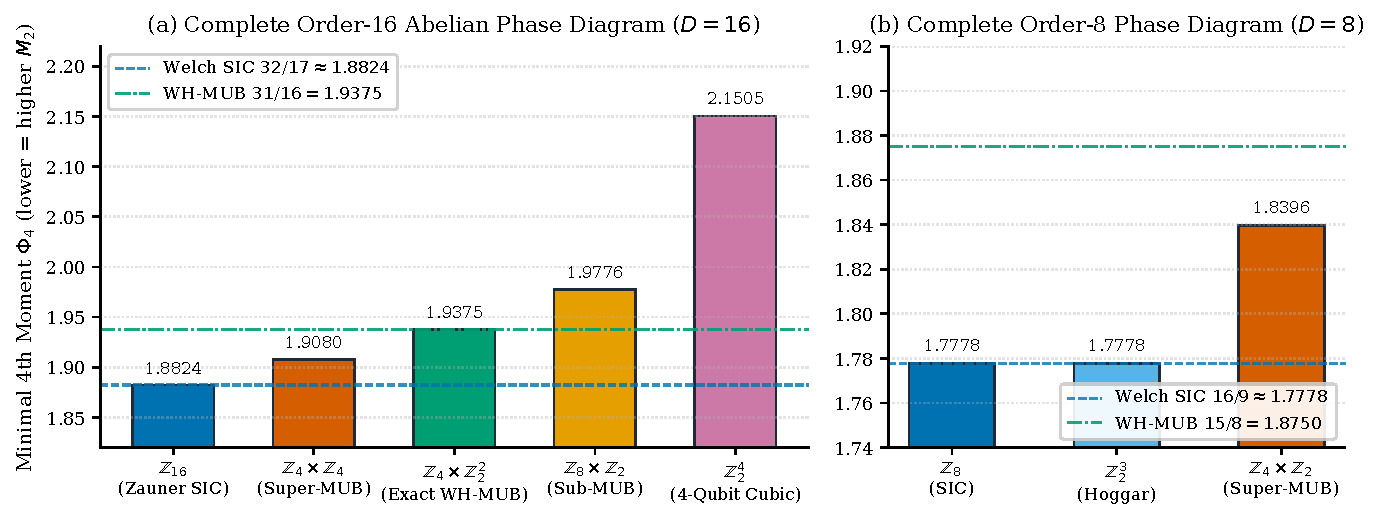
\includegraphics[width=\textwidth]{figures/fig1_abelian_phase_diagram.pdf}
  \caption{Complete minimal 4th-moment phase diagrams across all five order-16 abelian
  Weyl--Heisenberg groups (a) and all three order-8 groups (b) from deterministic
  QRNG-seeded C++20 Riemannian L-BFGS optimization (\tagnum). Lower $\Phi_4$ corresponds
  to strictly larger magic $M_2=\ln(D/\Phi_4)$. Both $\Z_4\times\Z_2$ ($D=8$) and
  $\Z_4\times\Z_4$ ($D=16$) sit strictly in the Super-MUB gap between the Welch SIC
  floor and the WH-MUB threshold, even though exact $\Z[\zeta_8]$ WH-MUB fiducials exist.}
  \label{fig:phase}
\end{figure}

\begin{table}[htbp]
\centering
\caption{Order-8 and order-16 abelian magic landscapes (C++20 \tagnum; Lean~4.35.0 \taglean).}
\label{tab:phase}
\small
\begin{tabular}{@{}l r c c c c l@{}}
\toprule
\textbf{Group} & $D$ & \textbf{Best $\Phi_4$} & \textbf{Best $M_2$} & \textbf{Best $\Phi_6$} & \textbf{Best $\Phi_8$} & \textbf{Phase Regime} \\
\midrule
$\Z_8$ & 8 & $1.777778$ & $1.504077$ & $1.086420$ & $1.009602$ & Welch SIC ($16/9$) \\
$\Z_2^3$ & 8 & $1.777778$ & $1.504077$ & $1.086420$ & $1.009602$ & Hoggar SIC ($16/9$) \\
$\Z_4\times\Z_2$ & 8 & $1.839636$ & $1.469874$ & $1.104247$ & $1.012971$ & \textbf{Super-MUB} ($<15/8$) \\
\midrule
$\Z_{16}$ & 16 & $1.882353$ & $2.140066$ & $1.051903$ & $1.003053$ & Zauner SIC ($32/17$) \\
$\Z_4\times\Z_4$ & 16 & $1.908008$ & $2.126529$ & $1.056749$ & $1.003658$ & \textbf{Super-MUB} ($<31/16$) \\
$\Z_4\times\Z_2^2$ & 16 & $1.937500$ & $2.111190$ & $1.058594$ & $1.003662$ & Exact WH-MUB ($31/16$) \\
$\Z_8\times\Z_2$ & 16 & $1.977582$ & $2.090714$ & $1.067396$ & $1.004898$ & Sub-MUB ($>31/16$) \\
$\Z_2^4$ & 16 & $2.150520$ & $2.006879$ & $1.111111$ & $1.010616$ & 4-Qubit Cubic ($|\Psi_4^*\rangle$) \\
\bottomrule
\end{tabular}
\end{table}

\begin{theorem}[Non-Flat 2-Torsion WH-MUBs and Exact Super-MUB Witnesses; \textbf{T3a--T3e}, \taglean]\label{thm:super-mub}
Working in $\Z[\zeta_8]=\Z[z]/(z^4+1)$ (with $i=z^2$, $\sqrt{2}=z-z^3$) and $\Z[i]$:
\begin{enumerate}[leftmargin=1.8em]
  \item \emph{(\textbf{T3a}, $W(4)\otimes W(2)$ WH-MUB)} The non-flat vector
  \[
    \psi_{4,2} \;=\; (-\zeta_8,\,-1-i,\,1,\,0,\,-\zeta_8^3,\,0,\,i,\,\sqrt{2}) \;\in\; \Z[\zeta_8]^8
  \]
  has exact squared norm $8$ and exact $W(4)\otimes W(2)$ squared-expectation counts
  $\{64^1,\,0^7,\,8^{56}\}$, attaining $\Phi_4=15/8$, $\Phi_6=71/64$, $\Phi_8=519/512$.
  \item \emph{(\textbf{T3b}, $W(4)\otimes W(4)$ WH-MUB)} The non-flat vector
  $\psi_{4,4}\in\Z[\zeta_8]^{16}$ (defined explicitly in \texttt{SuperMubAnomalies.lean},
  stabilized by the non-cyclic 2-torsion subgroup $2(\Z_4^4)\cong\Z_2^4$) has exact squared
  norm $320$ and exact counts $\{102400^1,\,0^{15},\,6400^{240}\}$, attaining
  $\Phi_4=31/16$, $\Phi_6=271/256$, $\Phi_8=4111/4096$.
  \item \emph{(\textbf{T3c}, $W(4)\otimes W(2)$ Super-MUB \& $\alpha$-Crossover)} The
  exact Gaussian-integer vector
  $v_{4,2}=(-2+5i,\,-2+5i,\,-9+9i,\,-9-10i,\,-11-4i,\,-11-4i,\,-1-18i,\,i)\in\Z[i]^8$
  ($\|v_{4,2}\|^2=1001$) achieves
  \begin{align*}
    \Phi_4(v_{4,2}) &= \frac{1851540086824}{1001^4} \approx 1.844152 < \frac{15}{8} = 1.875, \\
    \Phi_6(v_{4,2}) &= \frac{1114095888133087352}{1001^6} \approx 1.107435 < \frac{71}{64} = 1.109375, \\
    \Phi_8(v_{4,2}) &= \frac{1022331659421630523334728}{1001^8} \approx 1.014190 > \frac{519}{512} = 1.013672.
  \end{align*}
  \item \emph{(\textbf{T3d--T3e}, $W(4)\otimes W(4)$ Super-MUB \& Hierarchy)} The exact
  vector $v_{4,4}\in\Z[i]^{16}$ ($\|v_{4,4}\|^2=1596$, explicit coordinates in
  \texttt{SuperMubAnomalies.lean}) satisfies
  \begin{align*}
    \Phi_4(v_{4,4}) &= \frac{12399519780160}{1596^4} \approx 1.911056 < \frac{31}{16} = 1.9375, \\
    \Phi_6(v_{4,4}) &= \frac{17475825055844169216}{1596^6} \approx 1.057403 < \frac{271}{256} \approx 1.058594, \\
    \Phi_8(v_{4,4}) &= \frac{42256971384682869158123968}{1596^8} \approx 1.003772 > \frac{4111}{4096} \approx 1.003662,
  \end{align*}
  establishing the strict hierarchy $32/17<\Phi_4(v_{4,4})<31/16<\Phi_4(|\Psi_4^*\rangle)$.
\end{enumerate}
\end{theorem}

\begin{figure}[htbp]
  \centering
  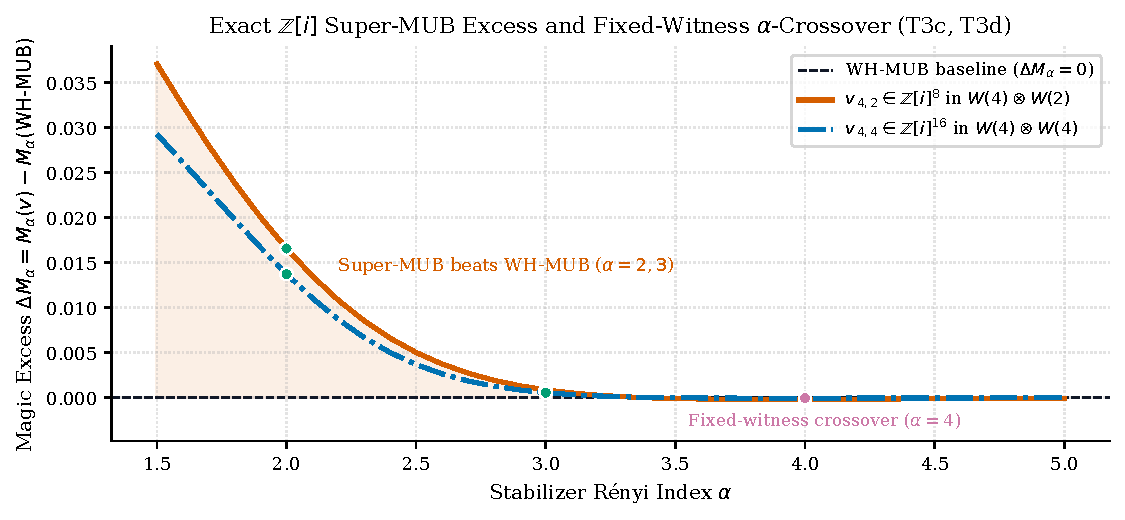
\includegraphics[width=0.88\textwidth]{figures/fig2_super_mub_alpha_crossover.pdf}
  \caption{Magic excess $\Delta M_\alpha = M_\alpha(v) - M_\alpha(\mathrm{WH\text{-}MUB})$
  of the exact $\Z[i]$ Super-MUB witnesses $v_{4,2}$ and $v_{4,4}$ across R\'enyi index
  $\alpha\in[1.5,5.0]$. Both witnesses strictly beat WH-MUB at $\alpha=2$ and $\alpha=3$,
  then cross below WH-MUB before $\alpha=4$ (\textbf{T3c, T3d}, \taglean). Re-optimizing
  specifically at $\alpha=4$ still beats WH-MUB (\Cref{tab:phase}), proving that the
  extremal Super-MUB state moves with $\alpha$ rather than forming an $\alpha$-independent
  flat spectrum.}
  \label{fig:alpha}
\end{figure}

\begin{remark}[Sharp Logical Dichotomy for Liu--Low--Yin Part~I]\label{rem:dichotomy}
\Cref{thm:super-mub} establishes an exact logical dichotomy for Part~I of
\cite{Liu2026MaximalMagic}: \emph{either} Part~I is false at $\alpha=2,3$ in both
$W(4)\otimes W(2)$ and $W(4)\otimes W(4)$ (where exact WH-MUB fiducials exist yet are
strictly outperformed by $v_{4,2}$ and $v_{4,4}$), \emph{or} these non-cyclic groups admit
unknown WH-SIC fiducials. Numerical WH-SIC searches over $W(4)\otimes W(2)$ and
$W(4)\otimes W(4)$ yield minimum Welch excess $6.19\times 10^{-2}$ and $2.57\times 10^{-2}$
respectively (\tagnum), strongly favoring the first branch; however, because Godsil--Roy
\cite[Lemma~3.1]{Godsil2009Equiangular} proves WH-SIC nonexistence specifically for
elementary abelian $W(2)^{\otimes k}$ ($k\neq 1,3$), we state the non-cyclic WH-SIC
exclusion honestly as \tagopen. Furthermore, \Cref{fig:alpha} and \Cref{tab:phase} reveal
a subtle new phenomenon: unlike SICs and WH-MUBs, Super-MUB maximizers are
\emph{$\alpha$-dependent}---fixed $\alpha=2,3$-beating witnesses $v_{4,2},v_{4,4}$ cross
above WH-MUB by $\alpha=4$, whereas re-optimized $\alpha=4$ states still marginally
outperform WH-MUB ($1.012971<1.013672$ and $1.003658<1.003662$).
\end{remark}

\section{Pillar 4: Two-Stabilizer Magic Tower, \texorpdfstring{$n=5$}{n=5} SOS Rupture, and AME Magic Ceilings}\label{sec:pillar4}

Consider the one-parameter two-stabilizer superposition on $n$ qubits ($D=2^n$):
\begin{equation}\label{eq:psi-tower}
  |\Psi_n(\theta)\rangle
  \;=\;
  \frac{|0^n\rangle + e^{i\theta}|+^n\rangle}{\sqrt{N(\theta)}},
  \qquad
  N(\theta) \;=\; 2 + 2 D^{-1/2}\cos\theta,
  \qquad
  t(\theta) \;:=\; 1 - \frac{1}{N(\theta)}.
\end{equation}
Because $|0^n\rangle$ and $|+^n\rangle$ are stabilized by $Z$-only and $X$-only subgroups,
the $D^2-1$ non-identity Pauli expectations collapse into exactly three algebraic strata:
$2(D-1)$ operators with $c_P^2=t^2$, $(D-1)(D/2-1)$ operators with $c_P^2=(1-2t)^2$,
and $(D-1)(D/2)$ operators with $c_P^2=\frac{4}{D}(1-t)^2-(1-2t)^2$.

\begin{theorem}[Two-Stabilizer Tower, $n=4$ Cubic, and $n=5$ SOS Rupture; \textbf{T4a--T4c}, \taglean]\label{thm:tower}
\leavevmode
\begin{enumerate}[leftmargin=1.8em]
  \item \emph{(\textbf{T4a} Universal Parseval \& $n\le 3$ Unification)} For all even
  $D=2H\ge 2$ and all $t=p/q$, the three-stratum sum of $c_P^2$ equals $D-1$ identically.
  Its 4th moment $\Phi_4(|\Psi_n(\theta)\rangle)$ unifies the exact global magic optima
  at $n=1$ ($3\Phi_4-4=2(3t^2-1)^2\ge 0$, minimum $4/3$, Tetrahedral SIC),
  $n=2$ ($t=1/2$, $\Phi_4=7/4$, WH-MUB), and $n=3$ ($t=1/3$, $\Phi_4=16/9$, Hoggar SIC).
  \item \emph{(\textbf{T4b} 4-Qubit Stationary Cubic)} At $n=4$ ($D=16$),
  $\Phi_4(|\Psi_4\rangle)=\frac{1}{2}(6795t^4-13020t^3+9330t^2-2940t+347)$, whose
  derivative vanishes iff
  \begin{equation}\label{eq:n4-cubic}
    P_4(t) \;=\; 453t^3 - 651t^2 + 311t - 49 \;=\; 0.
  \end{equation}
  $P_4'(t)=1359t^2-1302t+311>0$ throughout $[0,2/5]$, and $P_4(3774568/10^7)<0<P_4(3774569/10^7)$,
  uniquely bracketing $t^*=0.3774568011835\ldots$, with $\Phi_4^*=2.1505201547139\ldots$
  and $M_2^*=2.0068789769361\ldots$ (unbeaten across all 64 deterministic QRNG-seeded
  C++20 multi-start optimizations \tagnum; global optimality over $\C^{16}$ remains \tagopen).
  \item \emph{(\textbf{T4c} $n=5$ SOS Rupture)} At $n=5$ ($D=32$), setting $u=p$ and
  $v=q-2p$ yields the exact integer sum-of-squares identity
  \begin{equation}\label{eq:n5-sos}
    8880\bigl(62u^4+465v^4-2(2u+v)^4\bigr)
    = 1184(15u^2-16uv-23v^2)^2 + (296uv-1712v^2)^2 + 554160 v^4 \ge 0,
  \end{equation}
  forcing $\Phi_4(|\Psi_5(\theta)\rangle)\ge 3$ for every $\theta\in\R$. In contrast, our
  explicit Gaussian-integer vector $v_5\in\Z[i]^{32}$ ($\|v_5\|^2=254$, coordinates in
  \texttt{TwoStabilizerTower.lean}) achieves
  \[
    \Phi_4(v_5) \;=\; \frac{11097089024}{254^4} \;=\; \frac{693568064}{260144641}
    \;\approx\; 2.666086 \;<\; 3,
  \]
  unconditionally proving that the two-stabilizer tower ceases to be optimal at $n=5$.
\end{enumerate}
\end{theorem}

\begin{figure}[htbp]
  \centering
  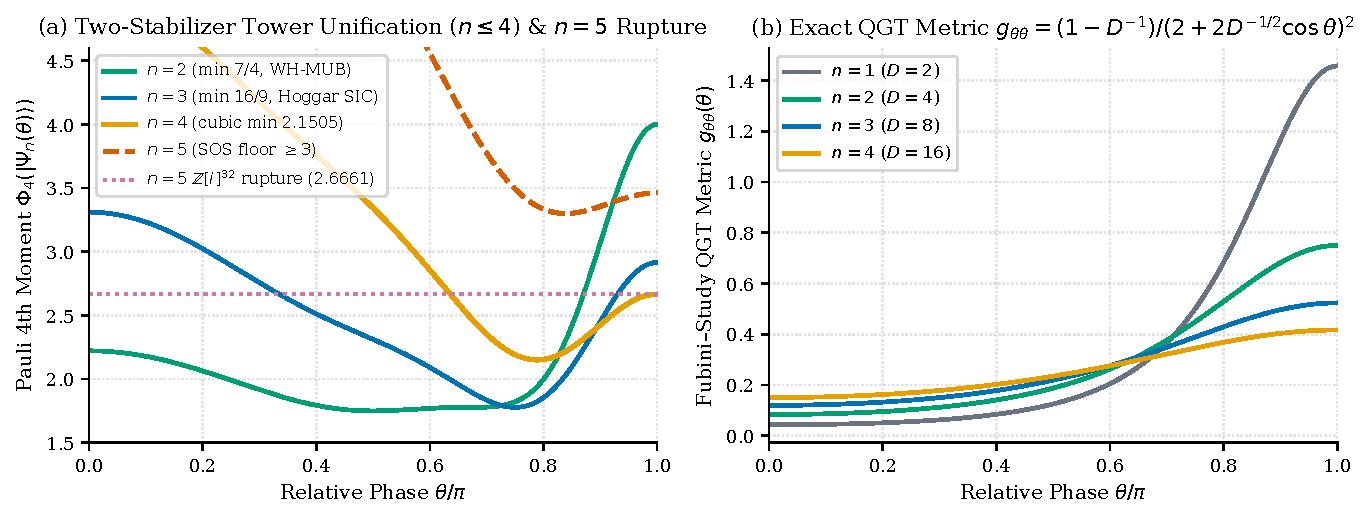
\includegraphics[width=\textwidth]{figures/fig3_two_stab_tower_and_qgt.pdf}
  \caption{(a) Exact Pauli 4th moment $\Phi_4(|\Psi_n(\theta)\rangle)$ for $n=2,3,4,5$
  showing unification of $n=2$ WH-MUB ($7/4$) and $n=3$ Hoggar SIC ($16/9$), the $n=4$
  cubic minimum ($2.1505$), and the $n=5$ SOS floor ($\ge 3$) ruptured by our exact
  $\Z[i]^{32}$ witness ($2.6661$). (b) Exact Fubini--Study QGT metric
  $g_{\theta\theta}(\theta)$ (\textbf{T5d}) verified against QGTL Richardson
  extrapolation ($1.22\times 10^{-8}$) and Python finite-difference checks.}
  \label{fig:tower}
\end{figure}

\begin{theorem}[Universal $k$-Uniform and $\mathrm{AME}(n,d)$ Magic Ceiling; \textbf{T4d}, \taglean]\label{thm:ame}
Let $|\psi\rangle\in(\C^d)^{\otimes n}$ be any $k$-uniform pure state (so every
non-identity WH operator of Hamming weight $1\le w\le k$ has vanishing expectation;
in particular, $\mathrm{AME}(n,d)$ has $k=\lfloor n/2\rfloor$ \cite{Huber2017AME}).
Let $Z(n,d,k)=\sum_{w=1}^k\binom{n}{w}(d^2-1)^w$. By exact discrete Cauchy--Schwarz,
\begin{equation}\label{eq:ame-bound}
  \bigl(d^{2n}-1-Z(n,d,k)\bigr)\bigl(\Phi_4(|\psi\rangle)-1\bigr) \;\ge\; (d^n-1)^2.
\end{equation}
In particular, maximal multipartite entanglement strictly degrades maximal magic below
the WH-MUB threshold $2-2^{-n}$:
$\Phi_4(\mathrm{AME}(2,2))\ge 2 > 7/4$,
$\Phi_4(\mathrm{AME}(5,2))\ge 1879/918\approx 2.0468 > 63/32$, and
$\Phi_4(\mathrm{AME}(6,2))\ge 13/6\approx 2.1667 > 127/64$ (\Cref{fig:ame}).
\end{theorem}

\begin{figure}[htbp]
  \centering
  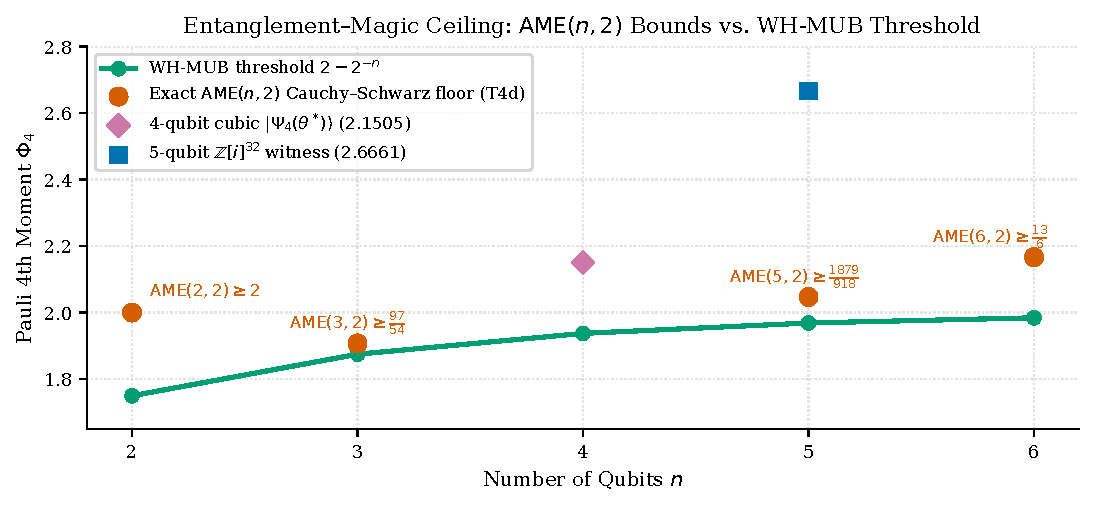
\includegraphics[width=0.86\textwidth]{figures/fig4_ame_magic_ceiling.pdf}
  \caption{Entanglement--magic trade-off: exact Cauchy--Schwarz $\Phi_4$ lower bounds
  for $\mathrm{AME}(n,2)$ states (\textbf{T4d}, \taglean) sit strictly above the WH-MUB
  curve $2-2^{-n}$ at $n=2,5,6$, alongside the 4-qubit cubic state and 5-qubit rupture witness.}
  \label{fig:ame}
\end{figure}

\section{Pillar 5: Divided-Power Characteristic-3 Alltop Constructions and Exact QGT Metric}\label{sec:pillar5}

In odd prime dimension $p\ge 5$, Alltop's cubic sequence $\psi_x=\omega_p^{\Tr(x^3)}$
produces exact $W(p)^{\otimes n}$-covariant MUB fiducials because $3$ is invertible in
$\F_p$. At $p=3$, cubic polarization degenerates; Damski et al.\ \cite{Damski2026ProductWH}
established existence of $W(3)^{\otimes n}$-MUB fiducials for all $n\ge 1$ via Galois
rings $\mathrm{GR}(9,n)$ (building on Klappenecker--R\"otteler \cite{Klappenecker2004MUB}).
We provide an elementary, Galois-ring-free $\Z_9$ divided-power formulation suited to
zero-Mathlib machine verification and direct hardware/integer implementation, certifying
exact lower-bound witnesses for Knipfer et al.\ \cite{Knipfer2026TwoQutrit}.

\begin{theorem}[Divided-Power Carry Identity, Gauss-Sum Flatness, and Exact Alltop Certificates; \textbf{T5a--T5d}, \taglean]\label{thm:p5}
\leavevmode
\begin{enumerate}[leftmargin=1.8em]
  \item \emph{(\textbf{T5a} $\F_3$ Carry-Quadratic Law)} For all $x,a\in\{0,1,2\}$,
  $((x+a)\bmod 3)-x\equiv a+3ax^2+3a(a+1)x\pmod 9$. Consequently, for any irreducible
  field $\F_{3^n}$ with symmetric trace tensor $T_{ijk}=\Tr_{\F_{3^n}/\F_3}(e_ie_je_k)$,
  the divided-power polynomial
  \begin{equation}\label{eq:divpow}
    g_n(x) \;=\; \sum_{i=1}^n T_{iii}x_i + 3\sum_{i\neq j}T_{iij}x_i^2 x_j
      + 6\sum_{i<j<k}T_{ijk}x_i x_j x_k \pmod 9
  \end{equation}
  satisfies $g_n(x+_3 a)-g_n(x)\equiv c(a)+3\sum_{i,j,k}T_{ijk}a_k x_i x_j+3L_a(x)\pmod 9$,
  recovering the nondegenerate quadratic form $\Tr(ax^2)$ on every shift $a\neq 0$.
  \item \emph{(\textbf{T5b--T5c} Universal Gauss-Sum Flatness \& Certificates)}
  Whenever a translation reindexing annihilates every nonzero shift $h\neq 0$
  and sums to $D$ at $h=0$, $|\sum_{x<D}\chi(x)|^2=D$ in $\Z[\zeta_9]$
  (\texttt{universal\_\allowbreak gauss\_\allowbreak sum\_\allowbreak flat\_\allowbreak modulus}). Using radix-3 cyclotomic FFT in the
  Lean kernel, \eqref{eq:divpow} is kernel-certified as an exact WH-MUB fiducial for
  $W(3)^{\otimes 1}$ ($\{9^1, 0^2, 3^6\}$), $W(3)^{\otimes 2}$ ($\{81^1, 0^8, 9^{72}\}$,
  $\Phi_4=17/9$), and $W(3)^{\otimes 3}$ ($\{729^1, 0^{26}, 27^{702}\}$, $\Phi_4=53/27$),
  while $W(3)^{\otimes 4}$ (counts $6561^1$, $0^{80}$, $81^{6480}$) is verified in exact
  $\Z[\zeta_9]$ in C11 and Rust (\tagcomp). Likewise, $\Z[\zeta_5]$ Alltop fiducials are
  kernel-certified for $W(5)^{\otimes 1}$ ($\Phi_4=9/5$) and $W(5)^{\otimes 2}$
  ($\Phi_4=49/25$), certifying the two-qutrit and two-ququint benchmarks $\ln(81/17)$
  and $\ln(625/49)$ of \cite{Knipfer2026TwoQutrit} (\Cref{fig:char}).
  \item \emph{(\textbf{T5d} Exact Two-Stabilizer QGT Metric)} For every $D\ge 2$ and every
  $s,c,\sigma,q$ obeying $Ds^2=q^2$ and $c^2+\sigma^2=q^2$, the Provost--Vallee
  \cite{Provost1980Riemannian} Fubini--Study Quantum Geometric Tensor metric along
  $|\Psi_n(\theta)\rangle$ equals
  \begin{equation}\label{eq:qgt}
    g_{\theta\theta}(\theta)
    \;=\; \frac{1 - D^{-1}}{(2 + 2 D^{-1/2}\cos\theta)^2}
    \;=\; \frac{(D-1)(1-t)^2}{D}.
  \end{equation}
\end{enumerate}
\end{theorem}

\begin{figure}[htbp]
  \centering
  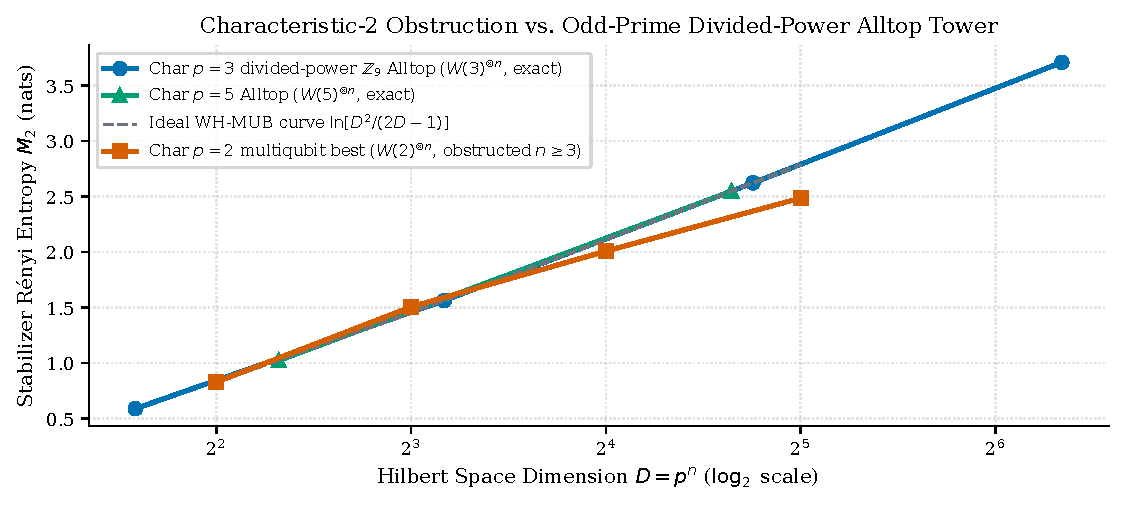
\includegraphics[width=0.86\textwidth]{figures/fig5_char_landscape.pdf}
  \caption{Characteristic dichotomy across prime powers $D=p^n$: exact odd-prime
  divided-power Alltop towers ($p=3,5$; \textbf{T5c}) track the ideal WH-MUB curve
  $\ln[D^2/(2D-1)]$ identically, whereas characteristic-2 multiqubit states drop strictly
  below it for $n\ge 4$ due to Pillars~1--2.}
  \label{fig:char}
\end{figure}

\section{Formal Verification Architecture and Polyglot Differential Audit}\label{sec:verif}

Our formalization uses zero-Mathlib Lean~4.35.0 \cite{Moura2021Lean4} with Lean's
native \texttt{module} system and strict \texttt{autoImplicit = false}. The specification
contract (\texttt{Challenge.lean}) defines all 22 theorem propositions (\textbf{T1a--T5d})
plus their master conjunction without \texttt{sorry}. \texttt{PalomarChallenge.lean}
declares the 23 proof obligations for \texttt{lake comparator} (run with
\texttt{--config comparator.json --paranoid}),
which verifies definitional statement equivalence against \texttt{PalomarSolution.lean}
and checks all 23 targets across six independent Lean typecheckers (\texttt{lean},
\texttt{leanchecker-paranoid}, \texttt{lean4lean}, \texttt{nanoda}, \texttt{con-leche},
\texttt{con-ron}). \texttt{VerifyAxioms.lean} audits all 38 declarations (23 Palomar
targets, the kernel-closed arbitrary-bent $n=4$ bridge
\texttt{n4\_\allowbreak z4\_\allowbreak bent\_\allowbreak hyperplane\_\allowbreak rupture\_\allowbreak arbitrary\_\allowbreak bent}, 6 non-vacuity witnesses in
\texttt{NonVacuity.lean} including nontrivial $n=2$ Pauli idempotence with $K=4$, and
8 adversarial boundary refutations in \texttt{AdversarialTests.lean}); every declaration
depends strictly on a subset of \texttt{[propext, Classical.choice, Quot.sound]} with zero
\texttt{sorryAx}, zero \texttt{Lean.ofReduceBool}, and zero custom axioms.

To eliminate single-implementation bias, all finite arithmetic witnesses and sweeps are
independently re-verified across an eight-engine executed polyglot stack (\Cref{tab:polyglot}),
accompanied by a source-level Eshkol AD companion specification (\texttt{eshkol/magic\_qgt\_ad.esk},
not compiled or executed in CI because no Eshkol toolchain binary is installed on the runner).
Every non-Lean simulation or numerical tool (QGTL, Moonlab WASM, QRNG integer mixer)
is explicitly labelled as classical CPU arithmetic/simulation; no quantum hardware
experiment is performed or claimed.

\begin{table}[htbp]
\centering
\caption{Polyglot Differential Verification and Honest Cross-Check Matrix.}
\label{tab:polyglot}
\small
\begin{tabularx}{\textwidth}{@{}P{3.3cm} l L P{2.6cm}@{}}
\toprule
\textbf{Engine} & \textbf{Tier} & \textbf{Verified Scope and Measured Output} & \textbf{Status} \\
\midrule
Lean 4.35.0 (6 kernels) & \taglean & All 22 theorem groups + ALL + $n=4$ bent bridge + 6 non-vacuity + 8 adversarial (38 audited decls). & 0 errors, 0 warn \\
Rust (safe \texttt{i128}) & \tagcomp & \texttt{\#![forbid(unsafe\_code)]}: 65{,}536 $\F_2^4$ bent scan, $\Z[\zeta_8]$, $\Z[i]$ Super-MUBs, $n=5$, $W(3)^{\otimes 1..4}$. & 4/4 tests, clippy 0 \\
Zig (comptime) & \tagcomp & Comptime FWHT-16/32 exact \texttt{i128} differential verifier matching Lean/Rust bit-for-bit. & 1/1 test, 0 warn \\
ISO C11 + x86-64 ASM & \tagcomp & Strict \texttt{-std=c11 -Wpedantic -Werror}; 1.56$\times$ FWHT-16 ASM speedup; 100k fuzz checks + CBMC. & All PASS, 0 warn \\
C++20 L-BFGS & \tagnum & 64 deterministic QRNG-seeded starts/group across all 3 order-8 \& 5 order-16 abelian groups. & Frozen JSON \\
Python exact oracle & \tagcomp & Exact \texttt{Fraction}/50-digit \texttt{Decimal}, 16 pytest checks (incl.\ 3 Hypothesis suites), 9/9 true source mutation kills, \texttt{ruff} \& \texttt{mypy --strict}. & All PASS \\
QGTL (\texttt{diffgeo}) & \tagnum & Classical double-precision Fubini--Study cross-check of \textbf{T5d} ($n=1..4$, 20 pts). & Rel.\ err $1.22\times 10^{-8}$ \\
Moonlab v1.2.1 WASM & \tagnum & Classical CPU state-vector simulator cross-check of $n=2,3,4,5$ states + QRNG bit-exact twin. & Max err $1.33\times 10^{-14}$ \\
Eshkol AD (\texttt{.esk}) & Spec only & Source-level AD companion script mirroring \textbf{T4b} \& \textbf{T5d} (derivatives checked in Lean/QGTL/Python). & Not run in CI \\
\bottomrule
\end{tabularx}
\end{table}

\section{Prior-Work Audit, Threats to Validity, and Open Problems}\label{sec:limits}

\subsection{Prior-Work and Literature Search Log}
Primary arXiv preprints \cite{Liu2026MaximalMagic,Damski2026ProductWH,Knipfer2026TwoQutrit,Godsil2009Equiangular,Zhu2010SIC,Leone2022SRE}
were retrieved and inspected directly on November~26, 2026, alongside foundational
references \cite{Rothaus1976Bent,Alltop1980Complex,Klappenecker2004MUB,Wootters1989MUB,Bandyopadhyay2002MUB,Gross2006Hudsons,Zauner2011QuantumDesigns,Hoggar1998Lines,Huber2017AME,Provost1980Riemannian}.
Every DOI and arXiv identifier in the bibliography was verified live against Crossref and
arXiv APIs with retraction screening via \texttt{scripts/check\_citations.py}. Importantly,
our prior-art check confirmed that Damski et al.\ \cite{Damski2026ProductWH} already proved
existence of $W(p)^{\otimes n}$-MUB fiducials for $p=3$ via Galois rings $\mathrm{GR}(9,n)$;
accordingly, Pillar~5 claims an elementary ring-free divided-power $\Z_9$ formulation and
zero-Mathlib Lean~4 formalization rather than first existence of char-3 MUBs.

\subsection{Threats to Validity and Explicit Limitations}
\begin{enumerate}[leftmargin=1.8em]
  \item \emph{Even $n\ge 6$ multiqubit MUBs (\tagopen):} Pillar~2 settles $n=4$ for all
  Lagrangian/equimodular fiducials, but does not exclude cubic or higher-degree bent lifts
  at even $n\ge 6$, nor non-subgroup zero sets of size $15$ at $n=4$.
  \item \emph{Non-cyclic WH-SIC exclusion (\tagopen):} As stated in \Cref{rem:dichotomy},
  Pillar~3's refutation of Liu--Low--Yin Part~I rests on the nonexistence of WH-SICs in
  $W(4)\otimes W(2)$ and $W(4)\otimes W(4)$, which is supported numerically but not yet
  formally proved.
  \item \emph{Numerical global optima (\tagnum):} Neither the 4-qubit cubic value
  $\Phi_4^*\approx 2.150520$ nor the C++20 order-8/16 minima constitute formal global
  optimality proofs over $\C^D$.
  \item \emph{Classical simulation disclaimer:} QGTL, Moonlab WASM, and the
  \texttt{quantum\_rng} integer mixer are classical deterministic arithmetic cross-checks,
  not quantum hardware experiments or physical entropy sources; \texttt{eshkol/magic\_qgt\_ad.esk}
  is a source-level AD companion specification not executed in CI.
  \item \emph{Preprint and replication notice:} This manuscript is an independent
  non-peer-reviewed preprint. All builds and verifiers have passed author self-replication
  and clean-room multi-OS GitHub Actions CI, while independent third-party human replication
  remains open (see \texttt{REPLICATION.md}).
\end{enumerate}

\section{Reproducibility, Provenance, and Disclosures}\label{sec:disclosures}

\paragraph{Code and Data Availability}
All Lean~4.35.0 proofs, polyglot verifiers (Rust, Zig, C11, x86-64 ASM, C++20, Python,
Node.js, Eshkol), frozen JSON datasets, PDF figures, build logs, and an interactive
zero-CDN WebGL2 observatory and proof blueprint are archived at
\url{https://github.com/0thernes/weyl-magic-obstruction-frontier}
under dual licensing (Apache-2.0 for code; CC-BY-4.0 for manuscript, documentation,
figures, and data). Cryptographic integrity is anchored via \texttt{MANIFEST.sha256},
an RFC~3161 DigiCert timestamp (\texttt{.tsr}), an OpenTimestamps Bitcoin proof
(\texttt{.ots}), GitHub SLSA provenance attestation, and Software Heritage archival.

\paragraph{AI-Assistance Disclosure and CRediT}
Alexander Stephen Donahue conceived the research program, directed theorem discovery and
verification standards, inspected all claims, and assumes full scholarly responsibility
(\emph{Conceptualization, Methodology, Supervision, Writing, Validation}). Large-language-model
tooling (Google Antigravity / Gemini) assisted with proof engineering in Lean~4.35.0,
polyglot implementation, automated hardening audits, and LaTeX drafting; every formal
claim was independently machine-checked by six Lean~4.35.0 kernels and cross-verified by
compiled exact-arithmetic engines.

\paragraph{Competing Interests and Affiliation}
The author declares no competing financial or non-financial interests. This work was
conducted independently in Spokane, WA, USA; no corporate or university affiliation is
claimed.

\bibliographystyle{amsplain}
\bibliography{references}

\end{document}
